%%%%%%%%%%%%%%%%%%%%%%%%%%%%%%%%%%%%%%%%%
% Stylish Article
% LaTeX Template
% Version 2.1 (1/10/15)
%
% This template has been downloaded from:
% http://www.LaTeXTemplates.com
%
% Original author:
% Mathias Legrand (legrand.mathias@gmail.com) 
% With extensive modifications by:
% Vel (vel@latextemplates.com)
% Final ACS by:
% Juan Barbosa
% License:
% CC BY-NC-SA 3.0 (http://creativecommons.org/licenses/by-nc-sa/3.0/)
%
%%%%%%%%%%%%%%%%%%%%%%%%%%%%%%%%%%%%%%%%%

\documentclass[fleqn,10pt]{SelfArx}

%----------------------------------------------------------------------------------------
%	ARTICLE INFORMATION
%----------------------------------------------------------------------------------------

\JournalInfo{Laboratorio Avanzado, No. 1, 20/4/2017} % Journal information
\Archive{ }

\PaperTitle{S\'intesis de Dilantin un antiepileptico a partir de benzaldehido} %
%\Keywords{Keyword1 --- Keyword2 --- Keyword3} % Keywords - if you don't want any simply remove all the text between the curly brackets
%\newcommand{\keywordname}{Keywords} % Defines the keywords heading name

%----------------------------------------------------------------------------------------
%	ABSTRACT
%----------------------------------------------------------------------------------------

\Abstract{\centering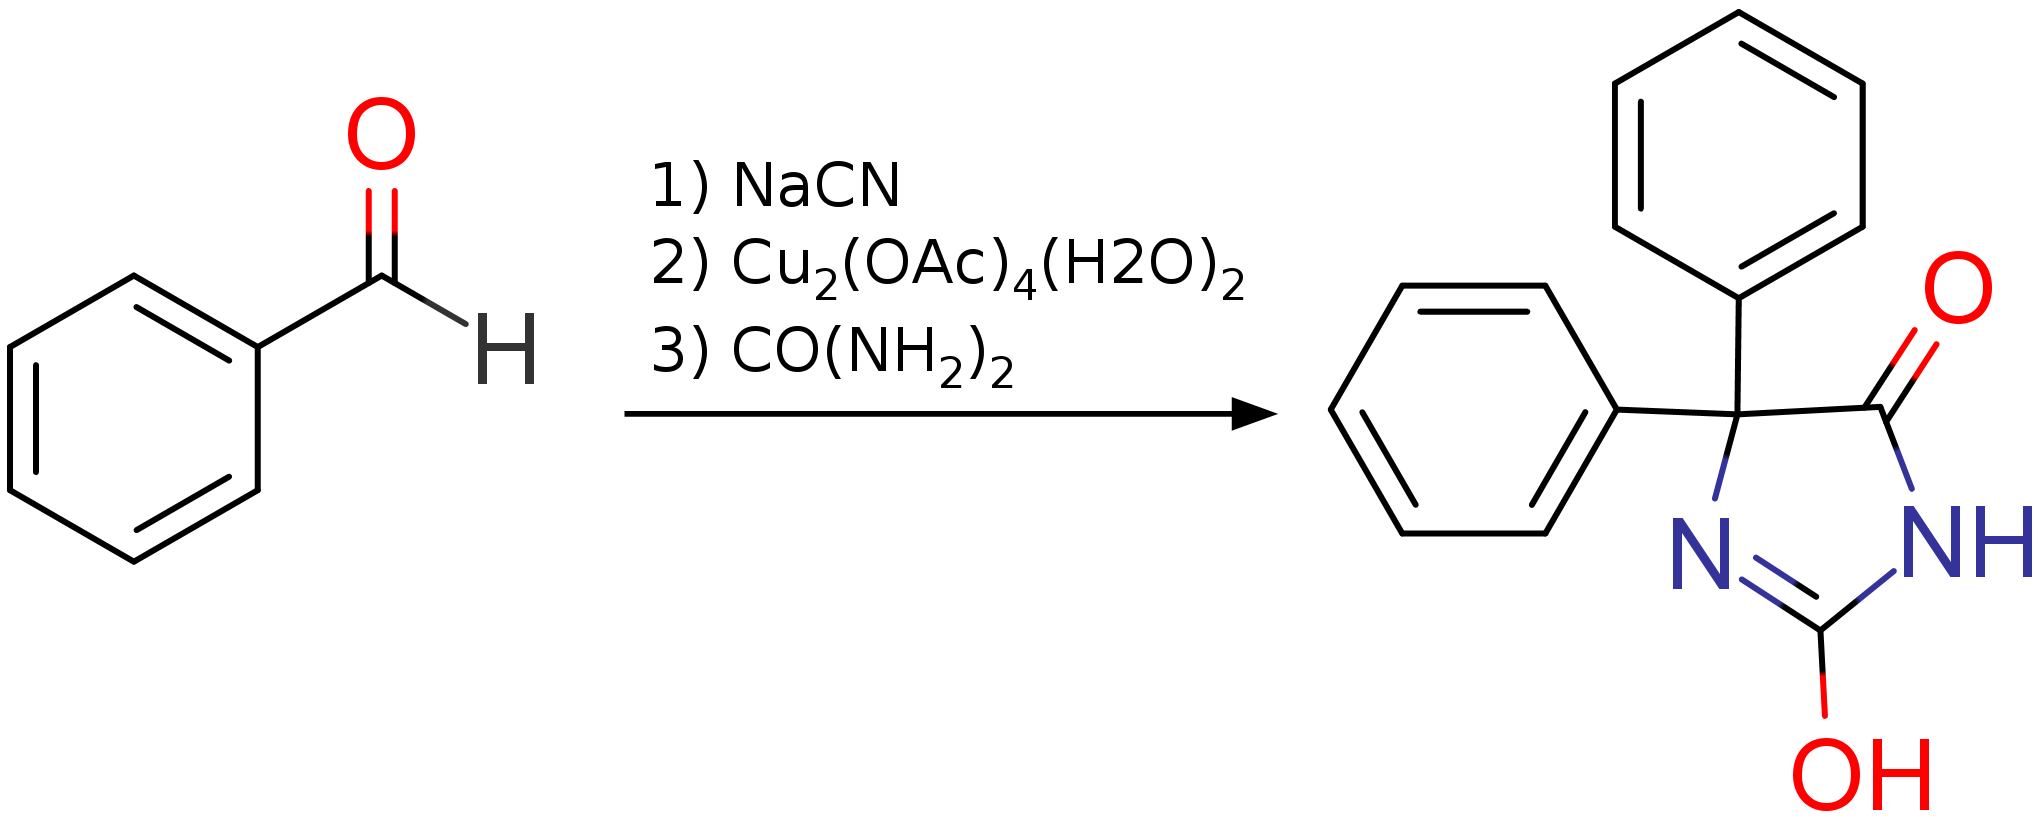
\includegraphics[scale=1]{structures/overall.png}}

%----------------------------------------------------------------------------------------

\begin{document}

\flushbottom % Makes all text pages the same height

\maketitle % Print the title and abstract box

%\tableofcontents % Print the contents section

\thispagestyle{empty} % Removes page numbering from the first page



%----------------------------------------------------------------------------------------
%	ARTICLE CONTENTS
%----------------------------------------------------------------------------------------

\section*{Introducci\'on} % The \section*{} command stops section numbering
Los compuestos de la familia de las hindanto\'inas son importantes medicamentos debido a su alta actividad biol\'ogica en el sistema nervioso central. A pesar que su principal uso es como antiepil\'eptico, tambi\'en es ampliamente usado como agente antiarr\'itmico, antitumor, bactericida y fungicida \cite{safari2010}. 

%------------------------------------------------

\section{Resultados y Discusi\'on}
\section{Conclusiones}
\section{Secci\'on experimental}
\subsection{S\'intesis de benzoina}
En bal\'on de reacci\'on fueron adicionados 7.0 mL de benzaldeh\'ido sin destilar (68.6 mmol), junto con 6.5 mL de etanol absoluto y 5.0 mL de una soluci\'on acuosa de cianuro de sodio M. Una trampa de bicarbonato de sodio en soluci\'on es usada para evitar la protonaci\'on del cianuro. La reacci\'on se lleva a reflujo por 40 minutos. El producto es filtrado y recristalizado en 65 mL de etanol.


\subsection{Oxidaci\'on}
La oxidaci\'on de la benzo\'ina se lleva a cabo usando 1.5004 g de acetato de cobre en 8.0 mL de una soluci\'on \'acido ac\'etico y agua (3/1 v/v). Los reactivos se agregan al bal\'on de reacci\'on y se lleva a reflujo en dos etapas de 20 minutos cada una. 
%----------------------------------------------------------------------------------------
%	REFERENCE LIST
%----------------------------------------------------------------------------------------
\phantomsection
\bibliographystyle{unsrt}
\bibliography{export}

%----------------------------------------------------------------------------------------

%\begin{figure*}[h]
%	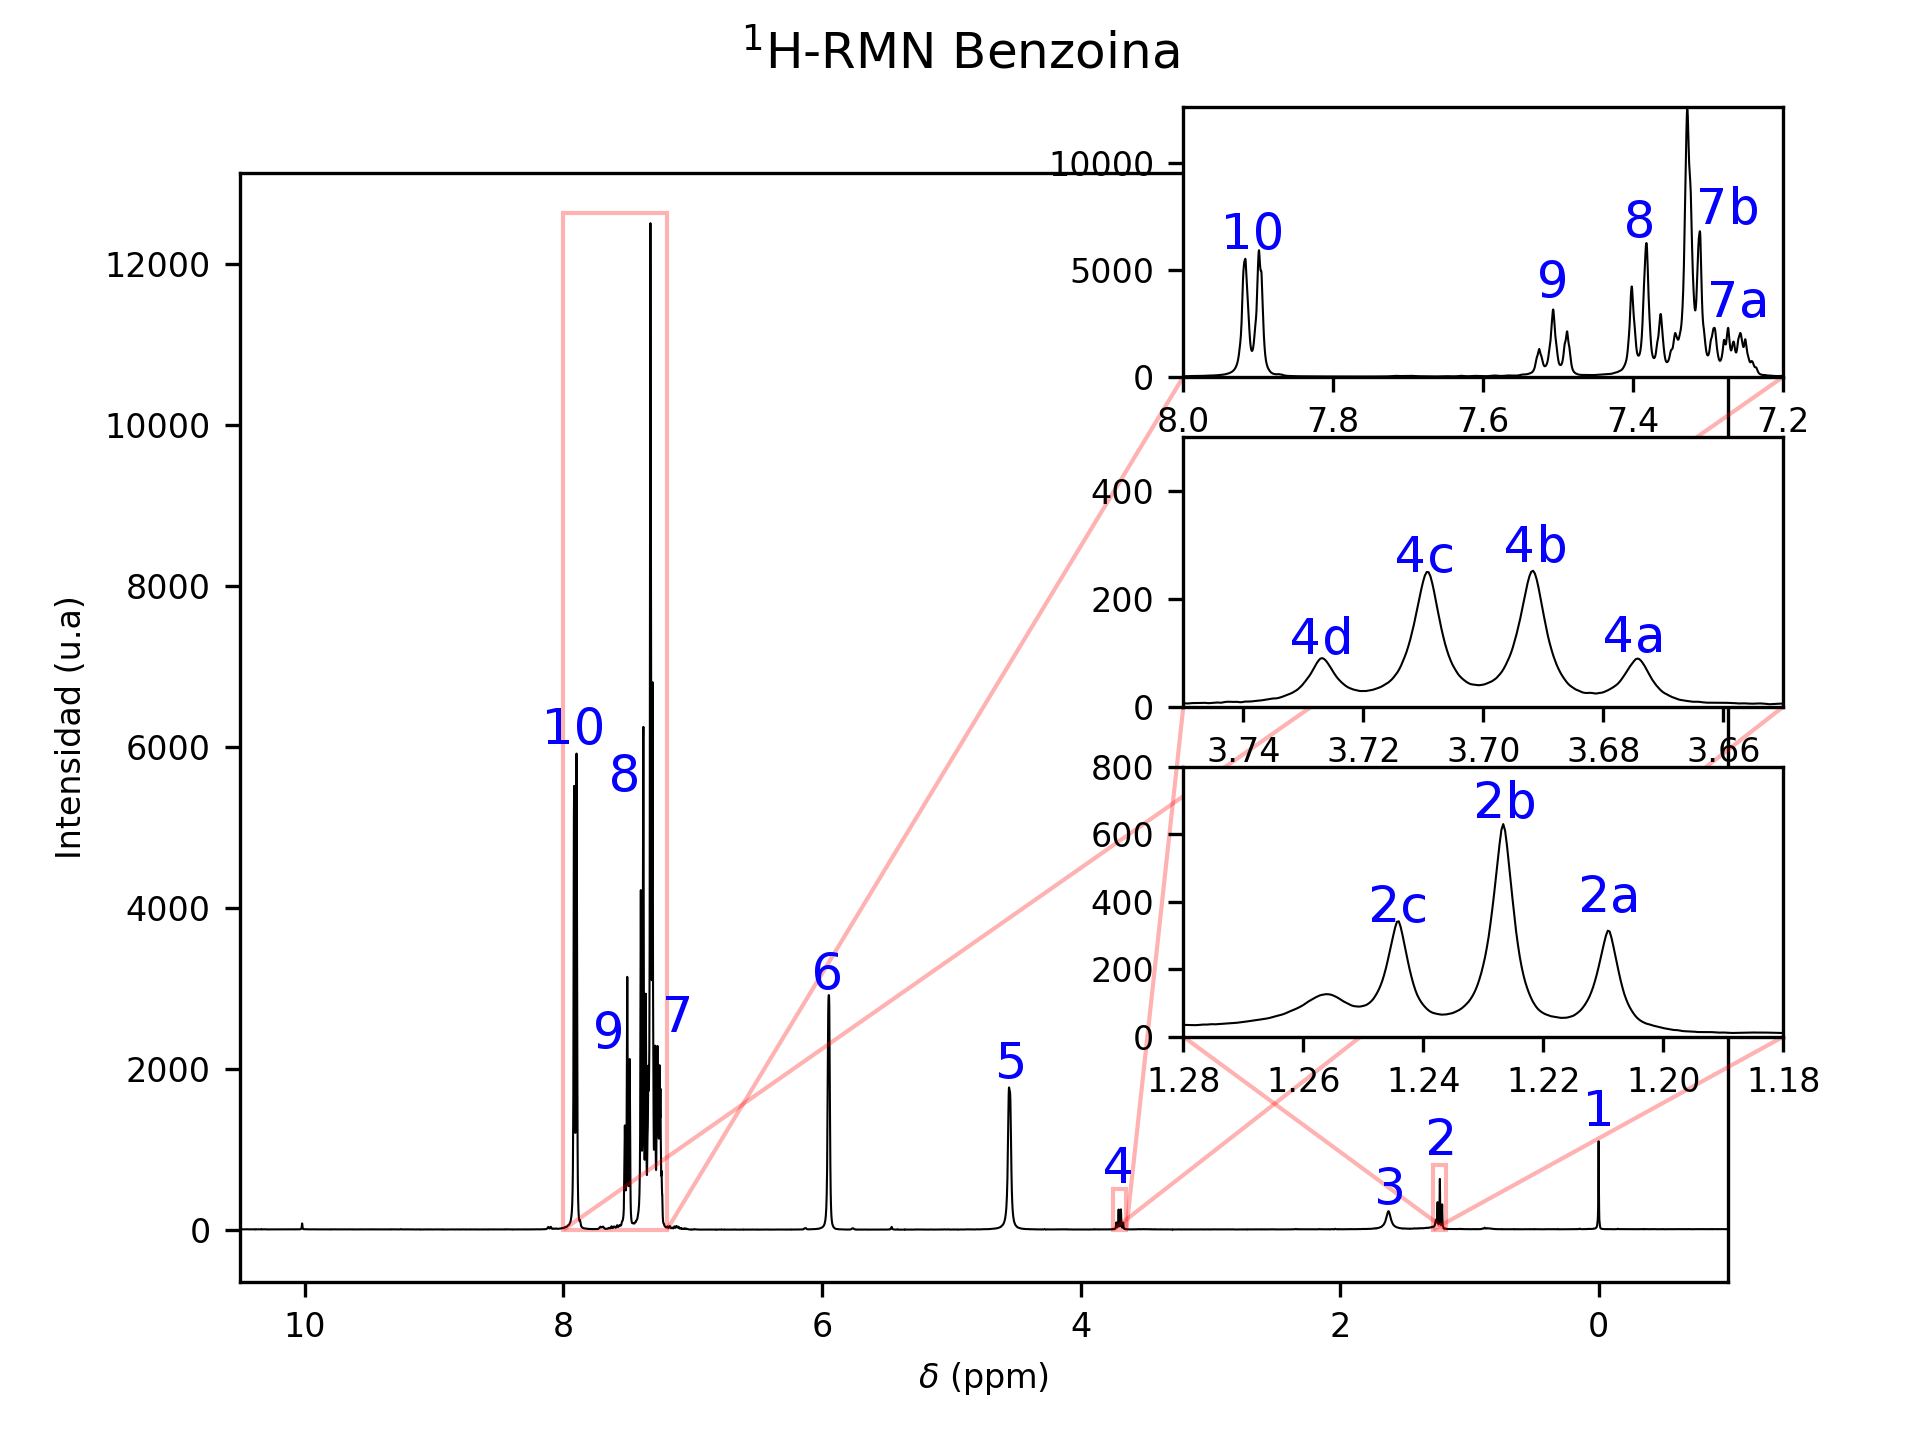
\includegraphics[width=\linewidth]{data/H-Benzoina-edited.png}
%\end{figure*}

\end{document}